\documentclass[11pt]{article}
\usepackage{enumerate}
\usepackage{fancyhdr}
\usepackage{amsmath}
\usepackage{graphicx}

\thispagestyle{empty}
\setlength{\parindent}{0cm}
\setlength{\parskip}{0.3cm plus4mm minus3mm}
\oddsidemargin = 0.0in
\textwidth = 6.5 in
\textheight = 9 in
\headsep = 0in

\title{CSCI 4100 Fall 2018 \\
% enter assignment number
Assignment 11 Answers}
\author{Damin Xu\\661679187}



\begin{document}
\maketitle
\newpage
% enter question #
\noindent{\bf Problem 1}
\begin{enumerate} [(a)]
	\item \ \begin{figure}[htb] 
			{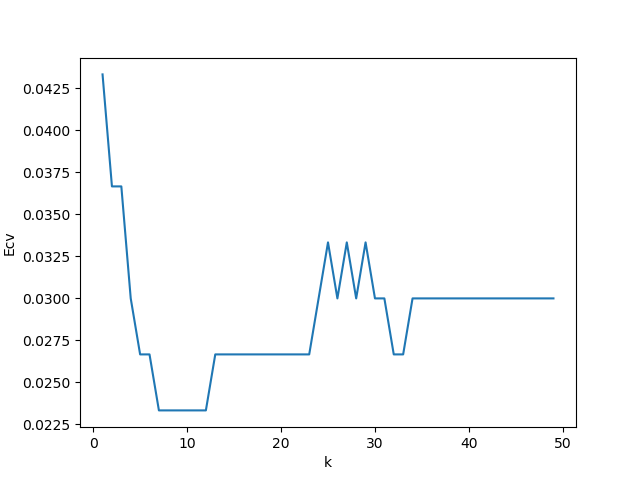
\includegraphics[height=8cm]{p1a.png}}
	\end{figure}
	I choose $k = 7$.
	\item \ \begin{figure}[htb] 
			{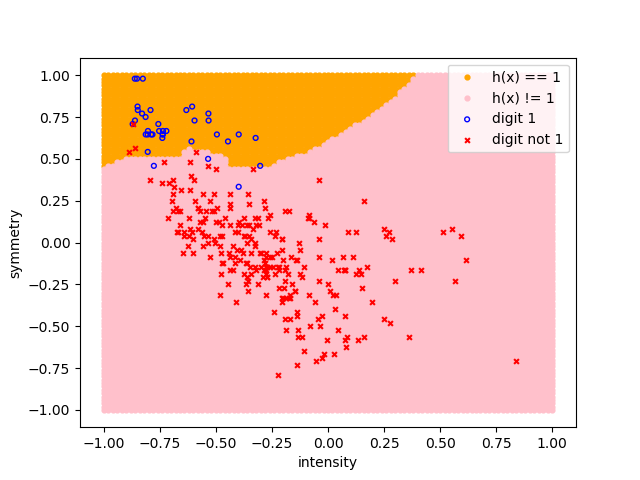
\includegraphics[height=8cm]{p1b.png}}
	\end{figure}
	$E_{CV} = 0.0233$ and $E_{in} = 0.02$

	\item $E_{test} = 0.0202267$
\end{enumerate}

\newpage
\noindent{\bf Problem 2}
\begin{enumerate} [(a)]
	\item \ \begin{figure}[htb] 
			{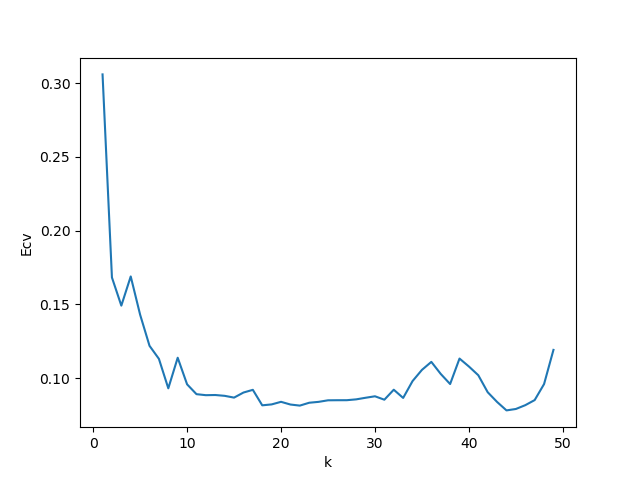
\includegraphics[height=8cm]{p2a.png}}
	\end{figure}
	I choose $k = 44$.
	\item \ \begin{figure}[htb] 
			{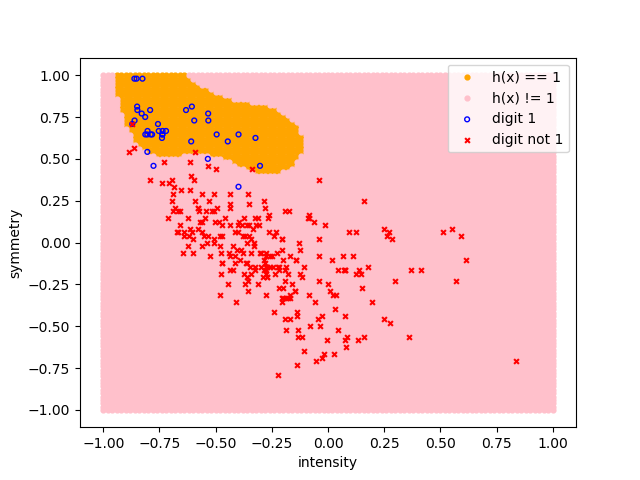
\includegraphics[height=8cm]{p2b.png}}
	\end{figure}
	$E_{CV} = 0.0782$ and $E_{in} = 0.02$
	\item $E_{test} = 0.0092242$
\end{enumerate}
\newpage
\noindent{\bf Problem 3} \\
$E_{test}$ for three methods:

\begin{tabular}{ll}
             & $E_{test}$ \\
KNN          & 0.0202267  \\
RBF          & 0.0092242  \\
Linear Model & 0.030669  
\end{tabular}

From the result above, KNN method have relatively similar $E_{test}$ to linear model with regularization. The reason is that KNN method follows the training data, and this is similar to linear model with high transformation. The RBF network performs much better than the KNN model because RBF network uses a large K value which is 44 whereas the K value used in KNN mdoel is only 7. Therefore, the decision boundary of RBF network is much strict than the KNN model and has a better $E_{test}$.
\end{document}
\end{document}
